\documentclass{article}
\usepackage{graphicx} % Required for inserting images
\usepackage{authblk} 
\usepackage{amsmath} 

\title{Resumen del Capítulo 2 de “Introduction To The Theory of Neural Computation” de Hertz, Krogh y Palmer (1991). Parte 3.}

\author{Rodrigo García Núñez}
\affil{Universidad Autónoma Metropolitana }
\date{Febrero 2025}


\begin{document}

\maketitle

\section{Función de Energía}
Como se dijo anteriormente, una de las contribuciones más importantes del trabajo de Hopfield (1982) fue la introducción de la función de energía a la teoría de las redes neuronales. Para las redes con las que trabajamos, representamos la función de energía de la siguiente forma:

\begin{equation}
    H  = -1/2 \sum_{ij}w_{ij}S_iS_j
    \label{Función de energía}
\end{equation}

Nótese que los términos en donde $i=j$ no son relevantes debido a que $S_{i}^2 = 1$, y en cualquier caso, podríamos escoger que $w_{ii} = 0$.
La función de energía es una función de la configuración $\{S_i\}$. Donde $\{S_i\}$ se refiere a todo el conjunto de todos los $S_i$'s. Se puede imaginar como un \textbf{superficie de energía} que está por encima del \textbf{espacio de configuraciones}. En la figura 1 se representa el espacio de configuraciones, y en la figura 2 se muestra la idea de la superficie de energía sobre el espacio de configuraciones.
\\
\begin{figure}
    \centering
    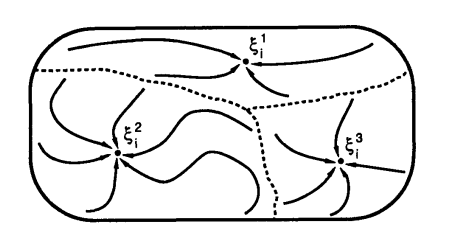
\includegraphics[width=0.5\textwidth]{images/EspacioConf.png}
    \caption{Espacio de configuraciones con atractores}
    \label{Espacio de configuraciones con atractores.}
\end{figure}


\begin{figure}
    \centering
    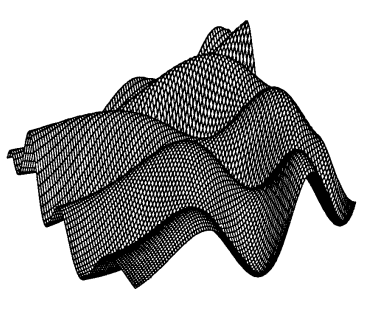
\includegraphics[width=0.5\textwidth]{images/SuperficieEnergia.png}
    \caption{Espacio de configuraciones con atractores}
    \label{Superficie de Energía.}
\end{figure}

La propiedad central de una función de energía es que siempre disminuye o se mantiene constante mientras el sistema evoluciona respecto a su regla dinámica. Los atractores presentes en la figura 1 son los mínimos locales de la superficie de energía. La dinámica puede ser pensada como algo similar a una partícula en la superficie de energía bajo la influencia de la gravedad (empujándola hacia abajo). Para cualquier punto de inicio de la partícula (siendo en este caso todo el estado $\{S_i\}$ del sistema), esta es tirada hacia abajo hasta posarse sobre alguno de los mínimos locales. Iniciando el sistema sobre alguna zona de atracción, el sistema recaerá en el atractor que corresponda a la zona.
\\\\
El término de \textbf{Función de energía} está inspirado en los sistemas magnéticos, de lo que se hablará más adelante. En muchos campos, hay una función que siempre se minimiza durante una evolución dinámica, o que debe ser minimizada para encontrar un estado óptimo y/o estable.

Para redes neuronales en general, la función de energía existe si la fuerza de las conexiones es simétrica, por ejemplo, $w_{ij} = w_{ji}$. En redes neuronales reales, esta no es una suposición razonable, pero es útil para estudiar el caso de la simetría dada la mayor información que la existencia de una función de energía provee. Para conexiones simétricas, podemos reescribir la ecuación 1 de la siguiente forma:
\begin{equation}
    H  = C - \sum_{(ij)}w_{ij} S_iS_j
    \label{Función de energía de conexiones simétricas}
\end{equation}
En donde $(ij)$ se refiere a todos los pares distintos de $ij$. Se excluyen los términos $ii$, pues de ellos sale la constante $C$.
Ahora es fácil notar que la regla dinámica
\begin{equation}
    S_i := sgn(\sum_jw_{ij}S_j)
    \label{modelo de la neurona}
\end{equation}
solo puede decrecer la energía. Por ejemplo, supongamos que $S_i^p$ es el nuevo valor de un $S_i$ dado por la regla dinámica para alguna unidad $i$, tal que

\begin{equation}
    S_i^p = sgn(\sum_j w_{ij}S_j)
    \label{actualización de $S_i$}
\end{equation}
Por un lado, si $S_i^p = S_i$, la energía no cambia. Por otro lado, si $S_i^p = -S_i$ y sacando los términos que involucran a $S_i$:

\begin{equation}
    H^p- H = - \sum_{j\neq i} w_{ij}S_i^pS_j + \sum_{j\neq i} w_{ij}S_iS_j  \\\\
    =2S_i\sum_{j\neq i}w_{ij}S_j \\\\
    = 2S_i \sum_j w_{ij}S_j - 2w_{ii}
    \label{}
\end{equation}
Debido a la ecuación 4, el primer término es negativo, y el segundo término también resulta negativo porque la regla de Hebb dice que $w_{ii}= p/N$ para todo i. Es así que la energía se reduce cada vez que $S_i$ cambia.
\\\\
Los términos acoplados a sí mismos $w_{ii}$ pueden ser omitidos completamente, ya que desde la regla de Hebb, pues podemos simplemente definir que $w_{ii}=0$, y del lado de la función de energía. Directamente se puede checar que esos términos no causan una diferencia importante a la estabilidad de $\epsilon_i^v$. Pero, lo que sí afecta es la dinámica y la cantidad de estados espurios (falsos/ilegítimos), por lo que resulta  mejor omitirlos [Kanter y Sompolinsky, 1987]. Podemos ver el porqué separando los términos autoacoplados de la regla dinámica:
\begin{equation}
    S_i := sgn(w_{ii}S_i + \sum_{j\neq i}w_{ij}S_j)
    \label{2.28}
\end{equation}
Si $w_{ii}$ fuese más grande que el segundo término en algún estado, entonces $S_i = +1$ y $S_i = -1$ serían ambos estables pues el segundo término no sería capaz de cambiar el signo del estado. Esto puede agregar más estados espurios estables al vecindario de algún atractor, reduciendo el tamaño de las zonas de atracción. 

\section{Iniciando desde una función de energía}
La idea de tener una función de energía como algo que queremos minimizar en los estados estables nos da una forma alternativa de aplicar la ley de Hebb. Lo que queremos es que la energía se reduzca cuando la similitud entre la configuración de la red y un estado almacenado sea mayor, tal que para el caso de un solo patrón almacenado
\begin{equation}
    H = - 1/2N (\sum_i S_{i}\epsilon_i)^{2}
    \label{2.29}
\end{equation}
Aquí, el factor $1/2N$ es el producto de una retrospectiva inspirada. Para el caso de varios patrones, podemos hacer que cada patrón $\epsilon_i^\mu$ sea un mínimo local de H, asumiendo lo de la ecuación 7 para todos los patrones:
\begin{equation}
    H = - 1/2N \sum_{\mu=1}^p(\sum_i S_{i}\epsilon_i^\mu)^{2}
    \label{2.30}
\end{equation}
y desarrollando
\begin{equation}
    H = - 1/2N \sum_{\mu=1}^p(\sum_i S_{i}\epsilon_i^\mu)(\sum_i S_{j}\epsilon_j^\mu) = - 1/2 \sum_{ij}(1/N\sum_{\mu=1}^p \epsilon_i^\mu\epsilon_j^\mu)S_iS_j
    \label{2.31}
\end{equation}
Lo que es exactamente igual a la función de energía original descrita en la ecuación 1, si $w_{ij}$ es dada por la regla de Hebb. 
Esta forma de encontrar los pesos $w_{ij}$ es muy útil. Si tenemos una función de energía cuyo mínimo satisface un problema de interés, entonces podemos desarrollarlo e identificar una sinapsis $w_{ij}$ apropiada desde el coeficiente de $S_iS_j$.
\section{Estados Espurios}
Se ha mostrado que la regla de Hebb, nos da un sistema dinámico que cuenta con atractores(para una cantidad de patrones p lo suficientemente pequeña) que funcionan como mínimos locales de la función de energía. Estos estados suelen llamarse \textbf{estados de recuperación}. Pero, como se dio indicios anteriormente, estos no son los únicos atractores.
Por un lado, se tiene que los estados inversos $-\epsilon_i^\mu$ son mínimos y comparten nivel de energía con los patrones originales, tal que la dinámica y la función de energía son perfectamente simétricas para todo i, $S_i \xleftarrow[]{}\xrightarrow[]{}-S_i$. No suponen un gran problema, pues podríamos invertir los bits restantes si algún bit bandera fuera -1, por ejemplo.
También hay \textbf{estados mezclados}  $\epsilon_i^{mix}$ que son estables, los cuales no son iguales a ningún patrón, sino que son combinaciones lineales de un número impar de patrones [Amit et al., 1985]. El caso más simple de estos estados es la combinación simétrica de 3 patrones almacenados, tal que
\begin{equation}
    \epsilon_i^{mix} =  sgn(\pm\epsilon_i^{\mu_1}\pm\epsilon_i^{\mu_2}\pm\epsilon_i^{\mu_3})
    \label{2.32}
\end{equation}
De esta ecuación, las 8 combinaciones de signos son posibles, pero por practicidad, analizamos el caso en que todos los signos son $+$, pues los demás casos son similares. Nótese que, en promedio, $\epsilon_i^{mix}$ tiene el mismo signo que $\epsilon_i^{\mu_1}$ tres veces de 4; solo si $\epsilon_i^{\mu_2}$ y $\epsilon_i^{\mu_3}$ tienen el signo opuesto, entonces puede que el signo de toda la expresión sea invertido. Entonces $\epsilon_i^{mix}$ tiene una distancia de Hamming de N/4 con los estados originales, por lo que el estado mezclado se ubica en puntos equidistantes de sus componentes. Esto implica que $\sum_i \epsilon_i^{\mu 1} \epsilon_i^{mix} = N/2$ en promedio. Para comprobar la estabilidad del estado compuesto, solo es necesario aplicar el cálculo de estabilidad para más de un patrón, pero es necesario sacar de la sumatoria los estados especiales $\mu$
\begin{equation}
    h_i^{mix} = 1/N \sum_{j\mu}\epsilon_i^{\mu}\epsilon_i^{\mu}\epsilon_i^{\mu} = 
    (1/2)\epsilon_i^{\mu_1}+(1/2)\epsilon_i^{\mu_2}+ (1/2)\epsilon_i^{\mu_3} + cross-terms
    \label{2.323}
\end{equation}
Es así que la condición de estabilidad se cumple para el estado compuesto.
\\\\
También se encuentran los \textbf{estados de vidrio de espín}, los cuales, para un $p$ grande, son mínimos locales que no están relacionados con cualquier número finito de estados $\epsilon_i^{\mu}$ [Amit et al., 1985b]. Estos reciben su nombre por la similitud con los modelos de vidrio de espín en el campo de la mecánica estadística.
\\\\
A los estados compuestos y a los estados de vidrio de espín se les conoce como \textbf{mínimos espurios}, en los que el sistema caerá si inicia cerca de alguno de ellos, pues tienden a tener zonas de atracción más pequeñas que las de los estados de recuperación. 

\section{Bibliografía}
\begin{thebibliography}{9}

\bibitem{John H., Anders K. y Richard G. P. (1992)} John H., Anders K. y Richard G. P. (1992). Introduction to the theory of Neural
Computation (pp. 17 - 20). CRC Press.
\end{thebibliography}
\end{document}
